\documentclass[12pt]{amsart}
%\documentclass[12pt]{article}

\usepackage{amsmath}
\usepackage{amssymb}
\usepackage{amsfonts}
\usepackage{euscript}
\usepackage{fancyhdr}
\pagestyle{fancyplain}
\usepackage{graphicx}
\usepackage{color}
\usepackage{txfonts}
 \usepackage{framed}
\usepackage{fancybox}


\topmargin=-2cm \oddsidemargin=-.5cm \evensidemargin=-1.5cm
\textwidth=17.2cm \textheight=25cm \onecolumn
\renewcommand{\baselinestretch}{1.51}





\newtheorem{ex}{Example}


\newtheorem{exer}{Exercise}

\newcommand{\s}{{\bf Solution. }}


\newcommand{\n}{   {\color{blue} $\clubsuit$  {\bf Note.}        }       }




%\shadowbox{ {\color{blue} $\clubsuit$  {\bf Note.} }{\it\large



\newcommand{\fm}{\mathfrak{M}}


%\chead{{\hspace{3.5cm} \bf bestmathtutor.ca Pre-Calculus   Subject: Graphing % }}
\lhead{Website: bestmathtutor.ca}   
\rhead{Contact Number: 778-882-4636} 




\begin{document}





\large

 %\fancyput(3in,-4.7in){\setlength{\unitlength}{1in}\fancyoval(7.5,10.7)}


  \fancypage{%
    \setlength{\fboxsep}{8pt}%
    \setlength{\shadowsize}{8pt}%
    \shadowbox}{}


\begin{center}
\textbf{To Graph $y=a\sin b(x-c)+d$
and $y=a\cos b(x-c)+d$}
\end{center}

%\begin{framed}

   
   \begin{itemize}
\item[\textbf{{\rm (1)}}] Draw the horizontal lines: $y=d-|a|,\;\;\;y=d,\;\;\;y=d+|a|;$  

\item[\textbf{{\rm (2)}}] Divide the interval $[c,\;\;c+\frac{2\pi}{b}]$ into 4 equal parts.  

\item[\textbf{{\rm (3)}}] The graph in one period is one of the following: 
\end{itemize} 
   
 \begin{center}
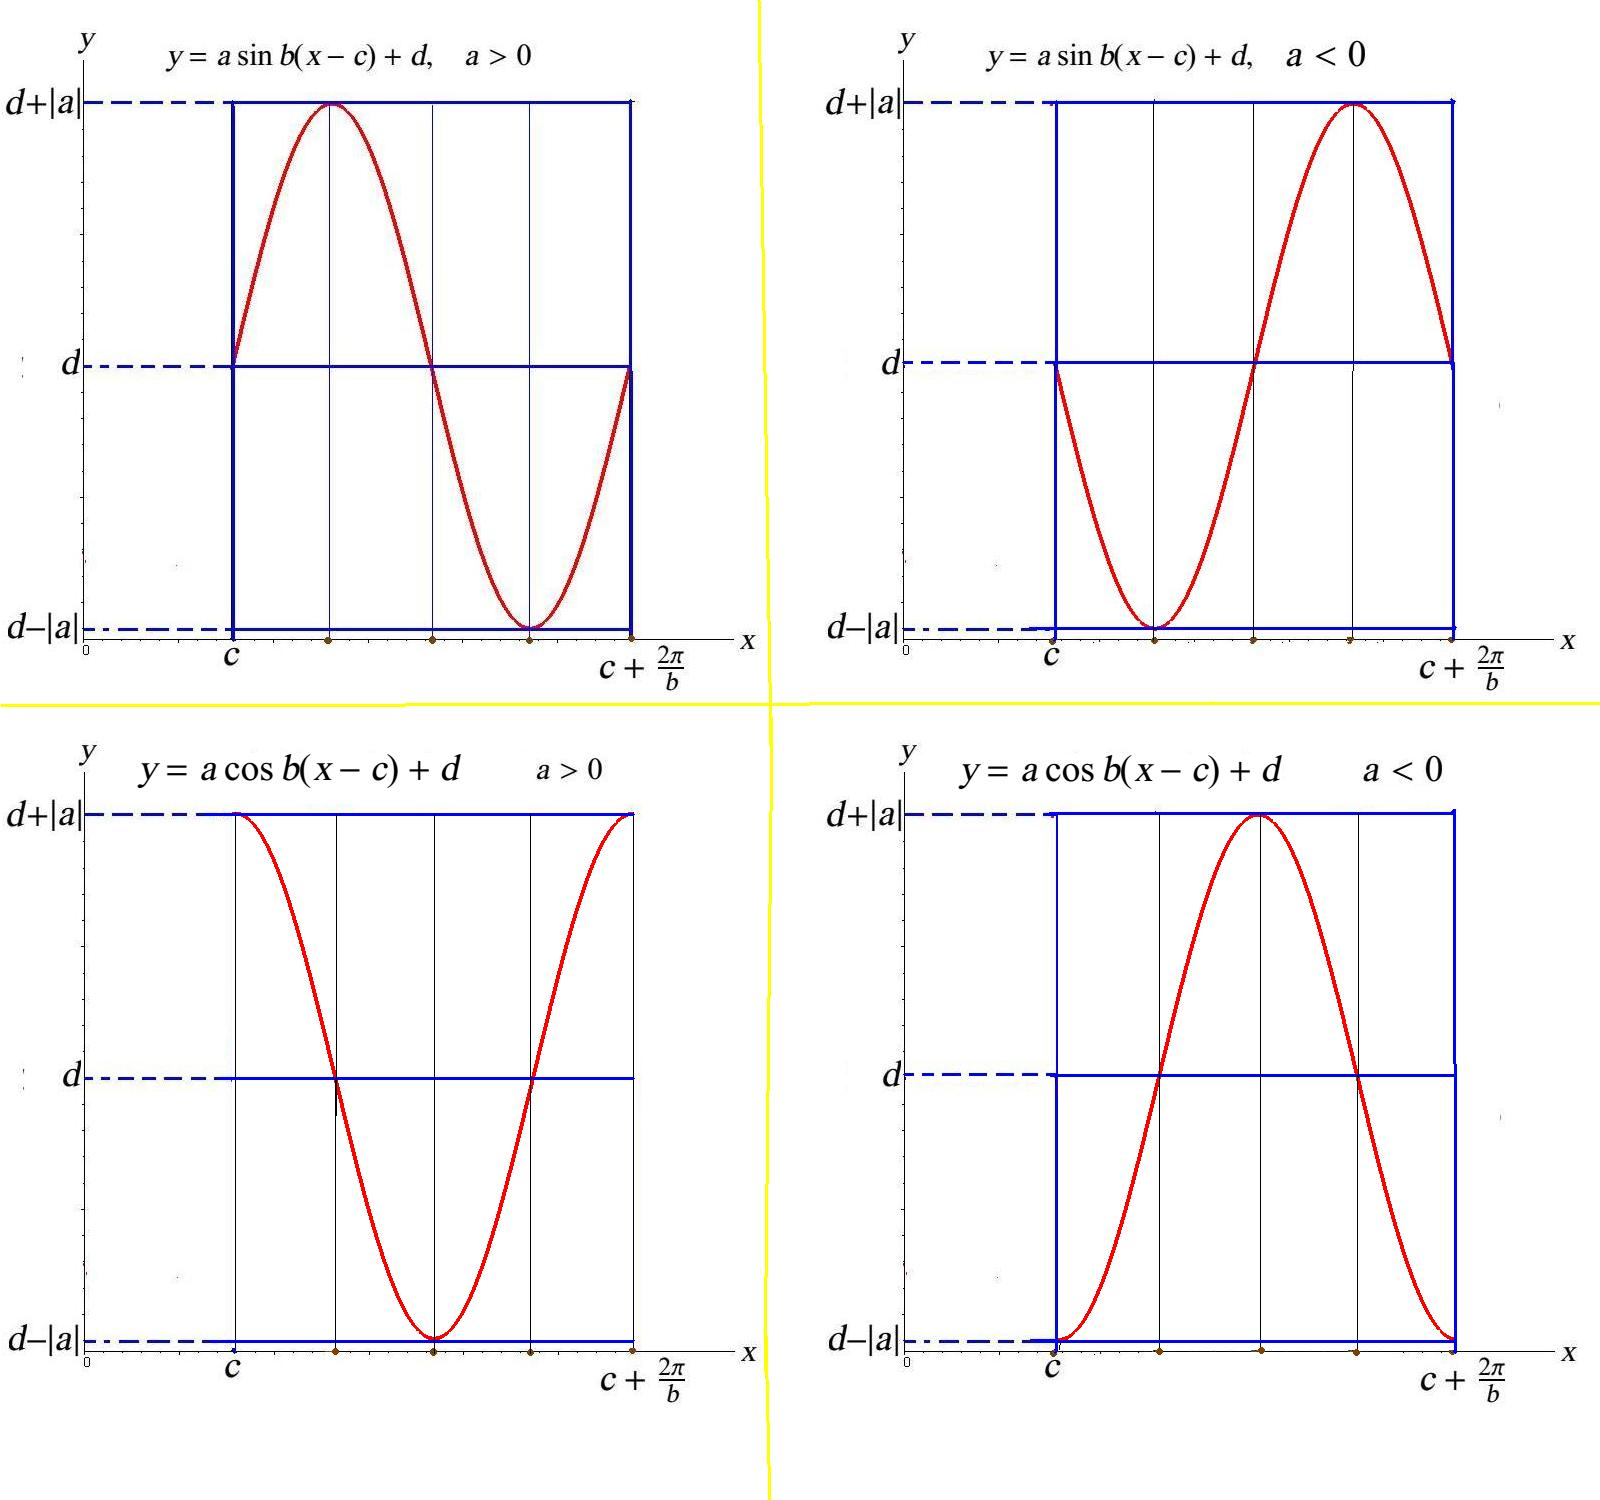
\includegraphics[height=5in, width=6in]{1}
\end{center}

%\newpage 
\begin{center}
\textbf{Finding the functions $y=a\sin b(x-c)+d$
and $y=a\cos b(x-c)+d$ from a graph}
\end{center}

\begin{itemize}
\item[\textbf{{\rm (1)}}] $a=\frac{Maximum-Minimum}{2},\;\;\; b=\frac{2\pi}{Period},\;\;\;d=\frac{Maximum+Minimum}{2};$

\item[\textbf{{\rm (2)}}] For the function of the form $y=a\sin b(x-c)+d,$ 
\\
$c=$ The x-coordinate of the intersection of the graph with the line $y=d$ such that the graph is above the line $y=d$ on the right side of this intersection point;

\item[\textbf{{\rm (3)}}] For the function of the form $y=a\cos b(x-c)+d,$ 
\\
$c=$ The x-coordinate of the intersection of the graph with the line $y=d+a.$ 
\end{itemize} 





\end{document}
